% ==============================================================================
% Copyright (c) 2017 [Georg R. Pollak]  
% ==============================================================================
% ------------------------------------------------------------------------------

  % Permission is hereby granted, free of charge, to any person obtaining a copy
  % of this software and associated documentation files (the "Software"), to deal
  % in the Software without restriction, including without limitation the rights
  % to use, copy, modify, merge, publish, distribute, sublicense, and/or sell
  % copies of the Software, and to permit persons to whom the Software is
  % furnished to do so, subject to the following conditions:

  % The above copyright notice, the creator of the formuary package G.R. Pollak
  % and this permission notice shall be included in all copies or substantial portions of the Software.

% ==============================================================================
% End
% ==============================================================================
% ------------------------------------------------------------------------------

% Document class
% ------------------------------------------------------------------------------
\documentclass[
  twoColumns,
  fontsize=10pt,
  baseClass=extarticle
]{formularyETH/formularyETH}
% formuaryETH packages
% ------------------------------------------------------------------------------
\usepackage{formularyETH/formularyETH_GeneralPackages}
\usepackage{formularyETH/formularyETH_underline}
\usepackage{formularyETH/extern/formularyETH_scientific}
\usepackage{formularyETH/extern/formularyETH_tikz}
%\usepackage{formularyETH/extern/formularyETH_coding}
\usepackage{formularyETH/extern/formularyETH_algorithms}
\usepackage{formularyMacros}
% -----------------------------math Formulary----------------------------------- 
% if git@gitlab.vis.ethz.ch:formularies/math.git is used as submodule
% ------------------------------------------------------------------------------
% Uncomment next line to obtain fallback macros for math
% \usepackage{math_submodule/formularyMacros} 
% And add next line to formulary
% \input{math_submodule/math.tex}
% Other very usefull packages
% ------------------------------------------------------------------------------
\usepackage[colorinlistoftodos,prependcaption,textsize=tiny]{todonotes}
%\usepackage[skip=0pt]{caption}
\usepackage[labelfont=bf]{caption}
\usepackage{wrapfig}
\usepackage{subcaption}
\usepackage{tabularx}
% In order to use inkscape figures with transparent fillings using alpha
\usepackage{transparent}
\usepackage{blindtext}
% -----------------------------Minted------------------------------------------- 
% minted uncomment next two lines
% ------------------------------------------------------------------------------ 
% \tcbuselibrary{minted}
% \tcbset{listing engine=minted}
% ------------------------------------------------------------------------------ 
% In emacs with auctex additionally add: 
% %%% TeX-command-extra-options: "-shell-escape"
% before %%% End
% -----------------------------Minted-end--------------------------------------- 
% ==============================================================================
% Documents Definitions title, date, ...
% ==============================================================================

\title{Deep Learning based Recommender Systems}

\author{
Tselepidis Nikolaos \\
\small{\texttt{ntselepidis@student.ethz.ch}}
    \and
Goetschmann Philippe \\
\small{\texttt{pgoetsch@student.ethz.ch}}
    \and
Maksimov Anton \\
\small{\texttt{antonma@student.ethz.ch}}
    \and
Pollak Georg Richard \\
\small{\texttt{pollakg@student.ethz.ch}}
}

\date{2020 January}
  % Graphic-paths important when including pdf_tikz pictures e.g. with inkscape
  % ------------------------------------------------------------------------------ 
  \graphicspath{{figures/}
                %{figures/ch1/}
          }
% ==============================================================================
% Document begin
% 1) Introduction
% Describe your problem and state your contributions.
% 2) Models and Methods
% Describe your idea and how it was implemented to solve the problem. Survey the related work, giving credit where credit is due.
% 3) Results
% Show evidence to support your claims made in the introduction. Compare to baselines / existing work.
% 4) Discussion
% Discuss the strengths and weaknesses of your approach, based on the results. Point out the implications of your novel idea on the application concerned.
% 5) Summary
% ==============================================================================
% ------------------------------------------------------------------------------
% Plots styles
% ------------------------------------------------------------------------------
\pgfplotscreateplotcyclelist{custom}{%
  plot_color_2, every mark/.append style={fill=plot_color_4, scale=1.2}, line width=2.5pt\\%
  plot_color_3,every mark/.append style={fill=plot_color_5, scale=1}, line width=2.5pt, densely dotted\\%
  plot_color_6,every mark/.append style={fill=plot_color_6, scale=1.8}, line width=2.5pt, dashed\\%
}
% ------------------------------------------------------------------------------
% Caption Set up
% ------------------------------------------------------------------------------
% \captionsetup[figure]{textfont={it}, labelformat=parens, labelsep=newline}
\begin{document}

\twocolumn[{%
  \begin{@twocolumnfalse} 
  \centering
  \maketitle
% Abstract
% ======================================================================
  \begin{abstract}
    \textbf{TODO: Finish abstract}
In this work, we conduct an empirical study of four recently proposed neural recommendation approaches, namely NCF \cite{he2017neural}, CMN \cite{ebesu2018collaborative}, NGCF \cite{wang2019neural}, and VAE \cite{liang2018variational}. Those engines can be used to solve collaborative filtering problems that rely on implicit feedback. The main motivation came from \cite{dacrema2019we} which states that there is a reproducibility crisis in the field of recommendation engines. To compare the aforementioned methods we adapted open source implementations to use equivalent metrics, preprocessing and train-test-splits on three different real-world datasets. Our results show that...
%%% Local Variables:
%%% mode: latex
%%% TeX-master: "../report"
%%% End:

  \end{abstract}
  \end{@twocolumnfalse}
  \vspace*{-3em}
}]

% Introduction
% ======================================================================
\section{Introduction}\label{sec:introduction}
Recommender systems are information filtering techniques that aim to predict the level of preference of a user over a specific item. 
In the era of big data, such techniques have attracted the interest of the scientific community, as they provide a natural approach to improving the user experience on various services, through personalization.
Classical recommender systems usually make use of either content-based or collaborative filtering approaches. 
Content-based filtering techniques utilize specific characteristics of an item in order to recommend additional items with similar properties, while collaborative filtering approaches utilize users' past behaviour i.e. preferences and interactions with items, as well as decisions of other users with similar interests. 
In most cases, collaborative filtering (CF) techniques yield improved predictions compared to the content-based approaches.
There are two main categories of methods when it comes to CF; (i) the Nearest-Neighbor techniques, and (ii) the Matrix Factorization (aka Latent Factor) methods.
As the Netflix Prize competition has demonstrated, Matrix Factorization methods are superior to classic Nearest-Neighbor techniques, as they allow the incorporation of additional information to the models, and can thus achieve improved model capacity \cite{koren2009matrix}.

Recently, both academia and industry have been in a race to design deep learning based recommender systems in an attempt to overcome the obstacles of conventional models and to achieve higher recommendation quality. 
In fact, deep learning can effectively capture non-linear and non-trivial user-item relationships, and also enable codification of more complex abstractions as data representations in the higher levels \cite{zhang2019deep}.
Various deep neural network architectures have been proposed and shown to be effective for predicting user preferences. 
Neural Collaborative Filtering (NCF) generalizes the Matrix Factorization (MF) approach by replacing the inner product utilized in MF models by a multi-layer perceptron that can learn non-linear user-item interaction functions, and thus increases the expressiveness of the MF model \cite{he2017neural}. 
Collaborative Memory Networks (CMN) unify the two classes of collaborative filtering models into a hybrid approach, combining the strengths of the global structure of the latent factor model, and the local neighborhood-based structure in a nonlinear fashion, by fusing a memory component and a neural attention mechanism as the neighborhood component \cite{ebesu2018collaborative}. 
Neural Graph Collaborative Filtering (NGCF) injects the collaborative signal into the embedding process by exploiting the user-item graph structure, so that it can effectively model high-order connectivity in the user-item interaction graph, and thus achieves improved recommendation quality \cite{wang2019neural}. 
Other deep learning based recommendation methods include Autoencoders, \cite{sedhain2015autorec}, Variational Autoencoders (VAE), \cite{liang2018variational}, and Restricted Boltzmann Machines (RBMs) \cite{salakhutdinov2007restricted}. 
However, as authors have stated in \cite{dacrema2019we} there has been a reproducibility issue with regards to neural recommendation approaches. 

In this work, we conduct an objective study of four recently proposed state-of-the-art neural network approaches, namely NCF \cite{he2017neural}, CMN \cite{ebesu2018collaborative}, NGCF \cite{wang2019neural}, and VAE \cite{liang2018variational}, that can be used in the context of collaborative filtering, on the basis of implicit feedback, in order to address the reproducibility crisis \cite{dacrema2019we}.
It should be stated, that implicit feedback reflects users' preference through behaviours like watching videos, purchasing products, and clicking items \cite{hu2008collaborative}.
As opposed to explicit feedback, i.e. ratings and reviews, implicit feedback can be tracked automatically, but is more challenging to utilize, since only user-item interactions are collected instead of user preferences.

In Section \ref{sec:models_and_methods}, we briefly present the aforementioned approaches along with the main underlying concepts.
In Section \ref{sec:results}, we give extensive comparative results of the selected approaches on three datasets from different application domains, i.e MovieLens (movie recommendations), cf. \cite{harper2016movielens}, Epinions (product recommendations), cf. \cite{epinions}, and Jester (joke recommendations), cf. \cite{jester}.
In Section \ref{sec:discussion}, we discuss the strengths and weaknesses of the selected methods based on the results, and finally in Section \ref{sec:summary} we summarize our work.

%%% Local Variables:
%%% mode: latex
%%% TeX-master: "../report"
%%% End:


% Models and Methods
% ======================================================================
\section{Models and Methods}\label{sec:models_and_methods}
\subsection{Neural Collaborative Filtering}\label{subsec:neural_collaborative_filtering}

The Neural Collaborative Filtering (NCF) approach \cite{he2017neural} is tightly related to the Matrix Factorization (MF) method \cite{koren2009matrix}, and provides a framework that is able to express MF and also generalize it.
Instead of simply ``combining'' the user and item latent vectors using a fixed inner product, NCF utilizes a multi-layer neural network architecture that learns the interaction function from the data, and thus, increases the expressiveness of the MF model.

An instance of the NCF framework takes as input two binary one-hot encoded vectors, one for the user, and one the item, and passes them through an embedding layer, i.e. a fully connected layer that projects the sparse representations onto dense vectors.
The obtained user and item embeddings can be viewed as the user and item latent vectors, respectively.
These vectors are then fed into a multi-layer neural network architecture, the output layer of which computes a predicted score $\hat{y}_{ui}$, for the specific user-item interaction.
This score represents how likely the item i is relevant to the user u.

Considering the one-class nature of implicit feedback, the value of $y_{ui}$ is being viewed as a label, where 1 means item relevant to u, and 0 otherwise.
Therefore, training is performed by minimizing the standard binary cross-entropy loss (a.k.a. negative log loss) between $\hat{y}_{ui}$ and its target value $y_{ui}$.
It should be noted, that in order to treat the problem as a binary classification problem and use the aforementioned loss function, negative instances are also required.
These instances are uniformly sampled from the unobserved interactions in each iteration.

In the paper \cite{he2017neural}, three instantiations of the NCF approach are considered, namely, the Generalized Matrix Factorization (GMF), the Multi-Layer Perceptron (MLP), and the Neural Matrix Factorization (NeuMF).
We briefly discuss them below.

\textbf{GMF:} Considering that the output of the embedding layer is the user and item latent vectors $p_u$ and $q_i$, respectively, we can define the mapping function of the first NCF layer as the element-wise product $p_u \odot q_i$.
We can then choose the output layer to be:
\begin{equation}
    \hat{y}_{ui} = \alpha_{out}(\vec{h}^{\T}(\vec{p}_{\idxu} \odot \vec{q}_{\idxi}))\label{eq:gmf}
\end{equation}
where $a_{out}$ and $h$ denote the activation function and affine transformation weights, respectively.
Setting $a_{out}$ to the identity and enforcing $h$ to be a uniform vector of 1, we can exactly recover the MF model.
In the GMF model, the authors set $a_{out}$ to the sigmoid function and learn the values of $h$ from the data with the log loss, effectively generalizing the MF approach.

\textbf{MLP:}
Instead of computing the element-wise product of the user and item latent vector, in a neural network framework it seems definitely intuitive to concatenate them, and then feed them into a standard MLP to learn the user-item interaction function.
In this way, much more flexibility and nonlinearity can be incorporated to the model, compared to the GMF approach, and increased expressiveness can be achieved. 
In \cite{he2017neural}, the authors utilize a tower pattern for the layers, halving the layer size for each successive layer.
As activation function the use ReLU in the middle layers, and sigmoid in the output layer.

\textbf{NeuMF:}
In the NeuMF model, the authors fuse the GMF and MLP approaches into a single architecture (see Fig. \ref{fig:neumf}) in an attempt to combine the linearity of MF and non-linearity of MLP, and thus to be able to better capture complex user-item interactions.
They even add more flexibility to the fused model by allowing GMF and MLP to learn separate embeddings.
In the last layer, the outputs of GMF and MLP are concatenated and are being fed into a sigle neuron with a sigmoid activation function.

\begin{figure}[t]
    \centering
    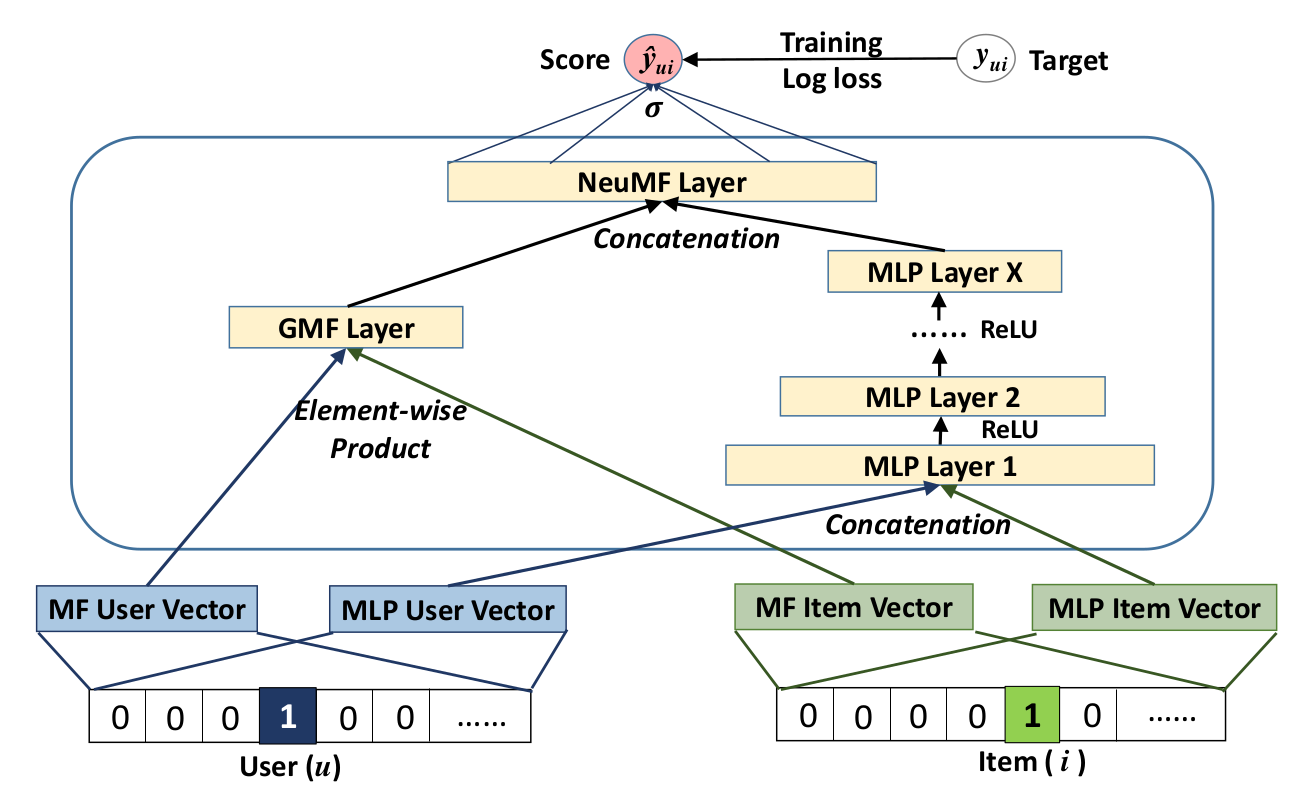
\includegraphics[width=0.8\linewidth]{images/neumf.png}
    \caption{Neural matrix factorization model taken from \cite{he2017neural}}
    \label{fig:neumf}
\end{figure}

%%% Local Variables:
%%% mode: latex
%%% TeX-master: "../../report"
%%% End:

\subsection{Collaborative Memory Network}\label{subsec:collaborative_memory_network}
\nospacing
The Collaborative Memory Network is a CF method and an extensions of NCF \cite{he2017neural} that tries to introduce 
localized user-item interactions using a neighborhood based approach by reweighting with an attention mechanism.
It contains three so called ``memory'' states, a user-, item-and a collective neighborhood memory-state:
Let $\idxi$ corresponds to the one-hot encoded item and $\idxu$ to the one-hot encoded user the user and item memory states are then defined by:
\begin{align*}
  \vec{m}_{\idxu}=\vec{M}\vec{\idxu}&&\vec{e}_{\idxi}=\vec{E}\vec{\idxi}&&\text{with}&&
   \begin{aligned}
    &\vec{\idxi}:=\unitVector_{\idxi}&&\vec{M}\in\R^{P\times d}\\[-1\jot]
    &\vec{\idxu}:=\unitVector_{\idxu}&&\vec{E}\in\R^{Q\times d}
   \end{aligned}                                                                         
\end{align*}
\subsubsection*{Output Model}
The attention mechanism allows to put attention on specific users withing the neighborhood that are similar to the current user of interest.
This weighting can be defined by calculating a user-preference vector $\vec{q}_{\idxu\idxi}$, where each dimension $v$ corresponds to
the endorsement of usre $v$ for item $\idxi$ plus the similarity with the target user $\idxu$: 
\begin{align*}
  \vec{q}_{\idxu\idxi v}&=\vec{m}_{\idxu}^{\T}\vec{m}_{v}+\vec{e}_{\idxi}^{\T}\vec{m}_{v} \qquad\forall v\in N(\idxi)
\end{align*}
the final weighting is then calculated by taking the softmax:\hfil$\vec{p}_{\idxu\idxi v}=\text{softmax}(\vec{q}_{\idxu\idxi v})$\\
This weighting is then used in order to calculate the collective neighborhood memory-state
\begin{align*}
  \vec{o}_{\idxu\idxi}=\sum_{\forall v\in N(\idxi)}\vec{p}_{\idxu\idxi v}\vec{c}_{v}&&\vec{c}_{\idxu}:=\vec{C}\idxu&&\vec{C}\in\R^{P\times d}
\end{align*}
The output/rating $\hat{r}_{\idxu\idxi}$ of the model for a given user and item is then given by:
\begin{align}
  &\vec{z}_{\idxu\idxi}=\phic\big(\overbrace{\vec{U}(\vec{m}_{\idxu}\odot\vec{e}_{\idxi})}^{\mathclap{\text{global use-item interaction}}}
  +\underbrace{\vec{W}\vec{o}_{\idxu\idxi}}_{\mathclap{\text{localized user-item-interactions}}}+\vec{b}\big)\quad\xrightarrow{\text{rating}}
  \hat{r}_{\idxu\idxi}=\vec{v}^{\T}\vec{z}_{\idxu\idxi}\nonumber \\[-1\jot]
  &\text{$W,U\in\R^{d\times d},v,b\in\R^d$ are trainable parameters.}
\end{align}
\begin{figure}[h]
  \centering
  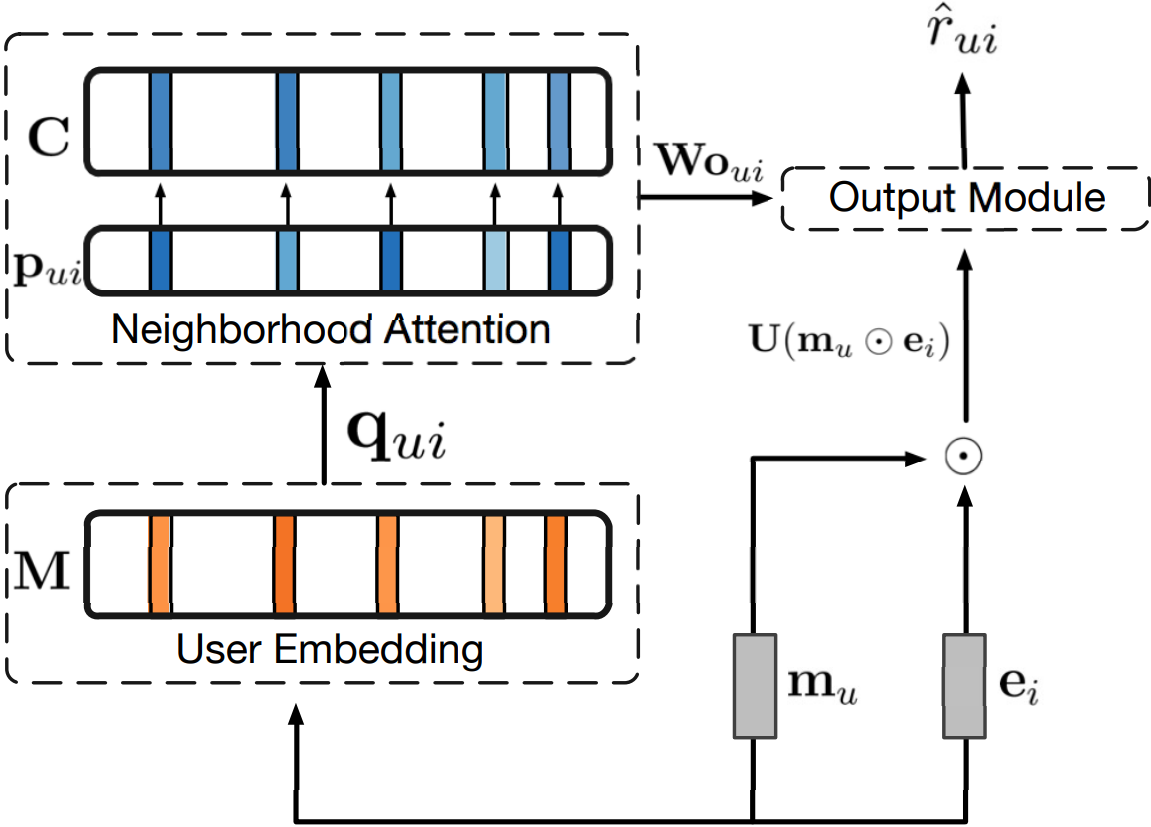
\includegraphics[width=0.7\linewidth]{figures/CMN.png}
  \caption{Schematic of the architecture taken from \cite{he2017neural}}
  \label{fig:}
\end{figure}
\subsubsection*{Multi-Hop Model}
\label{subsubsubsec:multi-hop}
Multiple of the memory models may be stacked together in order to improve the models predictability:
\begin{align}
  \vec{z}_{\idxu\idxi}^{t}=\phic\big(\vec{W}\vec{z}_{\idxu\idxi}^{t-1}+\vec{o}_{\idxu\idxi}^{t}
  +\vec{\mcb}^{t}\big)&&\text{with}&&\vec{z}_{\idxu\idxi}^{0}=\vec{m}_{\idxu}+\vec{e}_{\idxi}
\end{align}

%%% Local Variables:
%%% mode: latex
%%% TeX-master: "../../report"
%%% End:

\subsection{Neural Graph Collaborative Filtering}\label{subsec:neural_graph_collaborative_filtering}
\textbf{TODO: Summary by Anton}
%%% Local Variables:
%%% mode: latex
%%% TeX-master: "../../report"
%%% End:
\begin{figure}[h]
    \centering
    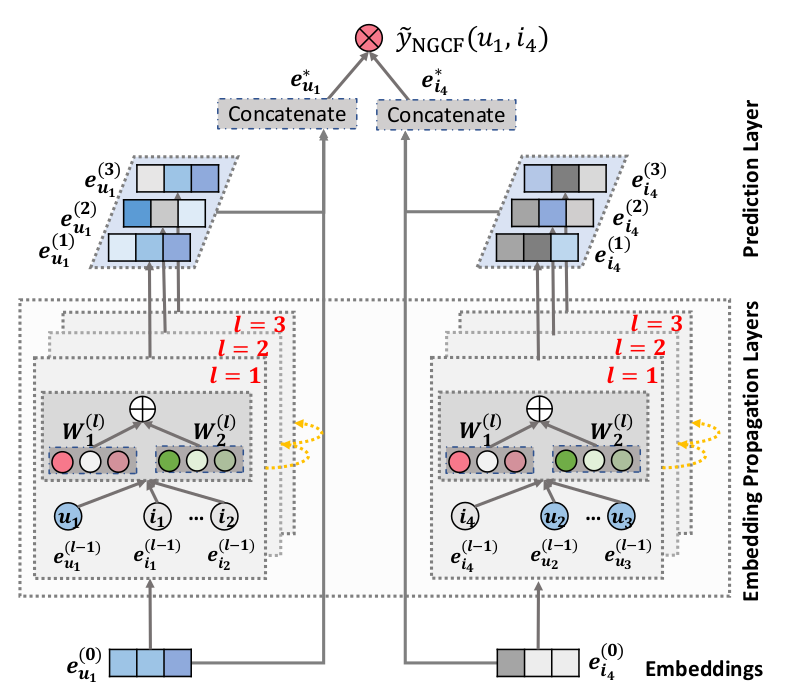
\includegraphics[width=0.8\linewidth]{images/ngcf.png}
    \caption{NGCF architecture.}
    \label{fig:ngcf}
\end{figure}

Tha main difference of NGCF \cite{wang2019neural} and NCF is the ``embedding propagation layers'', which are 
designed to incorporate collaborative signals.
\todo[inline]{Correct next senctence}
This signals include high-order connectivities in users-items connections graph, into embeddings of users and items \ref{fig:ngcf}.
\todo[inline]{TODO Stop}
Therefore, this is supposed to improve the quality of recommendations. 
Each layer corresponds to a measure of the distance between user and item interaction.
It produces messages which are passed between these graph nodes, summed and
\todo[inline]{change: result in embedding at this level.}
In the end all the embeddings for each level are concatenated in order to produce a final embedding.
\todo[inline]{Is this embedding plural or singular? in the next sentence}
This embedding plays the role of latent vectors which can simply be multiplied in order to obtain the rating.
The model is trained using pairwise BPR loss and optimized using Adam.
\subsection{Variational Autoencoder}\label{subsec:variational_autoencoder}
The original authors implement a variational autoencoder to solve collaborative filtering problems that are based on implicit feedback.

Variational autoencoders represent non-linear probabilistic models and can thus capture more complex relationships in the data than the linear factor models which are currently prevalent in collaborative filtering research.

They start by sampling a vector from a Gaussian distribution with $0$ mean and variance that corresponds to the number of items in the dataset. This sample is then transformed by a neural network to produce a probability vector over the items in the dataset where the probabilities should predict the users most likely next interaction. 

They use a multinomial likelihood to model the user's interaction history and empirically show that it outperforms gaussian and logistic likelihoods. 

For inference the parameters of the neural network have to be estimated and for this purpose the posterior distribution of the probability vector over items given a user and his interaction history needs to be calculated. This is not directly possible. As a solution the authors rely on variational inference which approximates the desired distribution through a fully factorized (diagonal) Gaussian distribution. Variational inference then tries to minimize the Kullback-Leiber divergence between the desired distribution and the surrogate. The new surrogate distribution grows in complexity with the number of users which might become problematic so the authors replace it's parameter by a data-dependent function (referred to as inference model) whose complexity only relies on the number of items in the data. This function introduces a new parameter $\phi$.

For learning, the log likelihood of the marginal data is lower bounded through the evidence lower bound which results in a loss function that depends on the parameters of the neural network and $\phi$. However, it's not trivially possible to take gradients with respect to $\phi$. To solve this issue the authors use the reparametrization trick which makes it possible to take the gradient with respect to $\phi$. Now it's possible to train the network with stochastic gradient descent.

To make predictions with a trained model, the user's interaction history is needed and put into a certain part of the inference model to calculate the input to the neural network which transforms it into a probability vector that predicts the probabilities with which items the user is most likely going to interact next. This means, given a new user, only two relatively efficient functions have to be called which makes predictions cheap.

%%% Local Variables:
%%% mode: latex
%%% TeX-master: "../../report"
%%% End:

\subsection{Ensemble}\label{subsec:ensemble}
For the ensemble method we combined the interaction probabilities of the other methods in the following way: each method generates a vector of interaction probabilities. Those probabilities can also be interpreted as rankings. To combine the rankings we gave weights to each rank. The lowest rank got a weight of 0, the second lowest rank a weight of 1, the third lowest rank a weight of 2 and so forth. To calculate the combined ranks we simply added up the weights given by each method for a particular item. For example, the item with the most added up weight would now have the highest combined rank. Then the combined ranks can now again be interpreted as interaction probabilities.

We choose this method because of it's simplicity and empirically it already delivers interesting results, however there are many ways how rankings or probability vectors can be combined and other methods might yield even better results.
%%% Local Variables:
%%% mode: latex
%%% TeX-master: "../../report"
%%% End:


% Results 
% ======================================================================
\section{Results}\label{sec:results}
\subsection{Experimental Setup}\label{subsec:experimental_setup}
\textbf{Datasets.}
We study the effectiveness of the aforementioned neural recommendation approaches on three publicly available datasets, i.e. Movielens \cite{harper2016movielens}, Jester \cite{jester}, and Epinions \cite{epinions}. 
The main characteristics of these datasets are summarized in Table \ref{tab:datasets}.

\begin{table}[h]
    \centering
    \begin{tabular}{c|c|c|c|c}
        \hline
        Dataset & \#Users & \#Items & \#Interactions & Density \\
        \hline
        Movielens &  6,040 &  3,706 & 1,000,209 & 0.0447 \\
        Jester    & 24,938 &    100 &   616,912 & 0.2474 \\
        Epinions  & 27,453 & 37,274 &    99,321 & 0.0001
    \end{tabular}
    \caption{Dataset statistics.}
    \label{tab:datasets}
\end{table}

Movielens is a movie rating dataset that has been widely utilized as a benchmark for evaluating collaborative filtering algorithms.
In our work, we use the version containing nearly one million ratings, where each user has rated at least 20 movies.
Jester, on the other hand, is a joke rating dataset with a lot more users, but a lot fewer items compared to Movielens.
We use the version where each user has rated between 15 and 35 jokes.
Epinions is a dataset containing consumer reviews for various products. 
This is a very sparse dataset, i.e. most of the users have rated very few items, a fact that leads to the existence of a very weak collaborative signal in the dataset. 
Therefore, Epinions is a very difficult benchmark for the selected methods, since all of them utilize the collaborative filtering effect, and thus, low quality recommendations are expected.

It should be stated, that although all the aforementioned datasets include explicit feedback from users, we transformed them into implicit feedback datasets in order to study the learning from the implicit signal.
To this end, we binarized the ratings, i.e. whenever there is a rating of a user to an item, either positive or negative, we set it to 1, since it denotes the existence of a user-item interaction. 
If there is no such interaction we set it to 0.

\textbf{Evaluation.}
We evaluate the quality of item recommendation using the leave-one-out evaluation method, following the prior work \cite{he2017neural,ebesu2018collaborative}.
In order to make the split as realistic as possible, for each user we held-out their latest interaction as the testset, and utilized the remaining data for training.
Then, we ranked the ``positive'' test item (i.e. item with the latest interaction by the user) against m randomly sampled ``negative'' items (i.e. items that this user has never interacted with).
We evaluated the ranking quality using the Hit Ratio (HR@k), and the Normalized Discounted Cumulative Gain (NDCG@k) metrics.
Intuitively, HR@k measures the presence of the ``positive'' item within the top k items, while NDCG@k measures the items' position in the ranked list, penalizing the score for ranking the item lower in that list.
We computed both metrics for each test user and for k=10, and reported the average score.

It should be stated, that since the Jester dataset does not include timestamps, we generated a random timestamp for each rating, and then proceeded to the train-test split. 
Moreover, it should be mentioned that for the case of Epinions, we filtered out from the dataset all the users that have only rated a single item, so as to avoid the cold-start setting (for the users).
Finally, for Movielens and Epinions we set m=99, while for Jester we set m=49, since there are only 100 items in the dataset in total, while there are users that have rated up to 35 items.

\subsection{Performance Comparison}\label{subsec:performance_comparison}
\textbf{TODO: }
\textit{Here we will present the tables and plots of the comparative results.}
\textit{Also state the methods' codenames. For example, Generalized Matrix Factorization with embedding size 8 has a codename GMF(8), Multilayer Perceptron with two layers will be called MLP(2), Neural Matrix Factorization with embedding size 8 and 2 layers will be called NeuMF(8,2) ... Something like that.}
\begin{table}[h]
    \centering
    \begin{tabular}{c|c|c}
        \hline
        Movielens & HR@10  & NDCG@10 \\
        \hline
        GMF(32)     & 0.7023 & 0.4202  \\
        MLP(4)      & 0.6616 & 0.3897 \\
        NeuMF(32,2) & 0.7012 & 0.4233 \\
        CMN         & 0 & 0 \\
        NGCF        & 0 & 0 \\
        VAE         & 0.7001 & 0.4230
    \end{tabular}
    \caption{Best performance achieved by each method (state configurations on codename) on Movielens dataset.}
    \label{tab:movielens}
\end{table}

\begin{table}[h]
    \centering
    \begin{tabular}{c|c|c}
        \hline
        Jester & HR@10 & NDCG@10 \\
        \hline
        GMF(16)    & 0.8411 & 0.7589 \\
        MLP(3)     & 0.8427 & 0.7569 \\
        NeuMF(8,2) & 0.8404 & 0.7563 \\
        CMN        & 0 & 0 \\
        NGCF       & 0 & 0 \\
        VAE        & 0.8482 & 0.7648
    \end{tabular}
    \caption{Best performance achieved by each method (state configurations on codename) on Jester dataset.}
    \label{tab:jester}
\end{table}

\begin{table}[h]
    \centering
    \begin{tabular}{c|c|c}
        \hline
        Epinions & HR@10 & NDCG@10 \\
        \hline
        GMF(64)     & 0.2348 & 0.1351 \\
        MLP(2)      & 0.3641 & 0.2135 \\
        NeuMF(32,2) & 0.3750 & 0.2167 \\
        CMN         & 0 & 0 \\
        NGCF        & 0 & 0 \\
        VAE         & 0.3503 & 0.2052
    \end{tabular}
    \caption{Best performance achieved by each method (state configurations on codename) on Epinions dataset.}
    \label{tab:epinions}
\end{table}

% Plot HR vs k, for best tuned models and for k=1,...,10, for all datasets
% \pgfplotstabletypeset{data.dat}

% Note about .dat file formating.
% Should have 3 columns, i.e.:
% k HR NDCG
% The k is ranging from 1 to 10.
% The respective Hit Ratios under HR.
% The respective NDCGs under NDCG.
\begin{figure*}[t]
    \centering
    %%%%%%%%%%%%%%%%%%%%%%%%%%%%%%%%%%%
    %%%%%% Hit Ratio - Movielens %%%%%%
    %%%%%%%%%%%%%%%%%%%%%%%%%%%%%%%%%%%
    \begin{subfigure}[ht]{0.3\textwidth}
        \centering
        \begin{tikzpicture}[scale=0.5]
        \begin{axis}[xlabel=k,ylabel=HR@k, legend pos=south east]
        \addplot table [x=k, y=HR]{results/movielens_gmf.dat};
        \addlegendentry{GMF(32)}
        \addplot table [x=k, y=HR]{results/movielens_mlp.dat};
        \addlegendentry{MLP(4)}
        \addplot table [x=k, y=HR]{results/movielens_neumf.dat};
        \addlegendentry{NeuMF(32,2)}
        \addplot table [x=k, y=HR]{results/movielens_ngcf.dat};
        \addlegendentry{NGCF(64)}
        \end{axis}
        \end{tikzpicture}
        \caption{Movielens}
    \end{subfigure}
    %%%%%%%%%%%%%%%%%%%%%%%%%%%%%%%%%%%
    %%%%%%% Hit Ratio - Jester %%%%%%%%
    %%%%%%%%%%%%%%%%%%%%%%%%%%%%%%%%%%%
    \begin{subfigure}[ht]{0.3\textwidth}
        \centering
        \begin{tikzpicture}[scale=0.5]
        \begin{axis}[xlabel=k,ylabel=HR@k, legend pos=south east]
        \addplot table [x=k, y=HR]{results/jester_gmf.dat};
        \addlegendentry{GMF(16)}
        \addplot table [x=k, y=HR]{results/jester_mlp.dat};
        \addlegendentry{MLP(3)}
        \addplot table [x=k, y=HR]{results/jester_neumf.dat};
        \addlegendentry{NeuMF(8,2)}
        \addplot table [x=k, y=HR]{results/jester_ngcf.dat};
        \addlegendentry{NGCF(32)}
        \end{axis}
        \end{tikzpicture}
        \caption{Jester}
    \end{subfigure}
    %%%%%%%%%%%%%%%%%%%%%%%%%%%%%%%%%%%%
    %%%%% Hit Ratio - Epinions %%%%%%%%%
    %%%%%%%%%%%%%%%%%%%%%%%%%%%%%%%%%%%%
    \begin{subfigure}[ht]{0.3\textwidth}
        \centering
        \begin{tikzpicture}[scale=0.5]
        \begin{axis}[xlabel=k,ylabel=HR@k, legend pos=south east]
        \addplot table [x=k, y=HR]{results/epinions_gmf.dat};
        \addlegendentry{GMF(64)}
        \addplot table [x=k, y=HR]{results/epinions_mlp.dat};
        \addlegendentry{MLP(2)}
        \addplot table [x=k, y=HR]{results/epinions_neumf.dat};
        \addlegendentry{NeuMF(32,2)}
        \addplot table [x=k, y=HR]{results/epinions_ngcf.dat};
        \addlegendentry{NGCF(8)}
        \end{axis}
        \end{tikzpicture}
        \caption{Epinions}
    \end{subfigure} 

    %%%%%%%%%%%%%%%%%%%%%%%%%%%%%%%%%%%%
    %%%%%%%%% NDCG - Movielens %%%%%%%%%
    %%%%%%%%%%%%%%%%%%%%%%%%%%%%%%%%%%%%
    \begin{subfigure}[ht]{0.3\textwidth}
        \centering
        \begin{tikzpicture}[scale=0.5]
        \begin{axis}[xlabel=k,ylabel=NDCG@k, legend pos=south east]
        \addplot table [x=k, y=NDCG]{results/movielens_gmf.dat};
        \addlegendentry{GMF(32)}
        \addplot table [x=k, y=NDCG]{results/movielens_mlp.dat};
        \addlegendentry{MLP(4)}
        \addplot table [x=k, y=NDCG]{results/movielens_neumf.dat};
        \addlegendentry{NeuMF(32,2)}
        \addplot table [x=k, y=NDCG]{results/movielens_ngcf.dat};
        \addlegendentry{NGCF(64)}
        \end{axis}
        \end{tikzpicture}
        \caption{Movielens}
    \end{subfigure}
    %%%%%%%%%%%%%%%%%%%%%%%%%%%%%%%%%%%
    %%%%%%%%%% NDCG - Jester %%%%%%%%%%
    %%%%%%%%%%%%%%%%%%%%%%%%%%%%%%%%%%%
    \begin{subfigure}[ht]{0.3\textwidth}
        \centering
        \begin{tikzpicture}[scale=0.5]
        \begin{axis}[xlabel=k,ylabel=NDCG@k, legend pos=south east]
        \addplot table [x=k, y=NDCG]{results/jester_gmf.dat};
        \addlegendentry{GMF(16)}
        \addplot table [x=k, y=NDCG]{results/jester_mlp.dat};
        \addlegendentry{MLP(3)}
        \addplot table [x=k, y=NDCG]{results/jester_neumf.dat};
        \addlegendentry{NeuMF(8,2)}
        \addplot table [x=k, y=NDCG]{results/jester_ngcf.dat};
        \addlegendentry{NGCF(32)}
        \end{axis}
        \end{tikzpicture}
        \caption{Jester}
    \end{subfigure}
    %%%%%%%%%%%%%%%%%%%%%%%%%%%%%%%%%%%%
    %%%%%%%%% NDCG - Epinions %%%%%%%%%%
    %%%%%%%%%%%%%%%%%%%%%%%%%%%%%%%%%%%%
    \begin{subfigure}[ht]{0.3\textwidth}
        \centering
        \begin{tikzpicture}[scale=0.5]
        \begin{axis}[xlabel=k,ylabel=NDCG@k, legend pos=south east]
        \addplot table [x=k, y=NDCG]{results/epinions_gmf.dat};
        \addlegendentry{GMF(64)}
        \addplot table [x=k, y=NDCG]{results/epinions_mlp.dat};
        \addlegendentry{MLP(2)}
        \addplot table [x=k, y=NDCG]{results/epinions_neumf.dat};
        \addlegendentry{NeuMF(32,2)}
        \addplot table [x=k, y=NDCG]{results/epinions_ngcf.dat};
        \addlegendentry{NGCF(8)}
        \end{axis}
        \end{tikzpicture}
        \caption{Epinions}
    \end{subfigure} 
    \caption{Evaluation of top k item recommendation, where k ranges from 1 to 10 on the three datasets.}
\end{figure*}

%%% Local Variables:
%%% mode: latex
%%% TeX-master: "../../report"
%%% End:


%%% Local Variables:
%%% mode: latex
%%% TeX-master: "../report"
%%% End:

\subsection{Comments}\label{subsec:results_comments}
\textbf{TODO: }
\textit{Technical comments, difficulties, or implementation details regarding the results.}

% VAE
\textbf{On train/validation/test-splits for the variatioal autoencoder:} in the implementation for the variational autoencoder, the original authors have done their train/validation/test-splits slightly differently: They splitted the users in respective groups instead of excluding some interactions for each user. For our comparison this way of splitting was not possible because some methods need to train embeddings for their users. As a result, the Hit-Ratio and NDCG that were generated with the validation split on the variational autoencoder did not agree with the Hit-Ratio and NDCG that our test-split generated. The validation metrics became worse as we trained for more epochs, however the test metrics became better. To not let the variatonal autoencoder underperform we decided to tune the number of epochs according to the test-split. This also suggests that we are indeed overfitting on the users we are training on (which is also on what the test metrics are evaluated). This might or might not be desired in a real-world application.

\textbf{Parameter tuning for the variational autoencoder:} the original authors state that annealing is quite important for the performance so we tried different largest annealing parameters ranging from 0.0 to 1.0 but neither validation- nor test-metrics were influenced by it.

% Ensemble
\textbf{Ensemble:} unfortunately it was not trivial to generate the necessary ranking matrices to feed into the Ensemble-method. We could not include the Collaborative Memory Networks because debugging them took days of computing time and also for the variational autoencoder there was a bug which lead to slight deviations between the results directly obtained after training and reevaluating the generated ranking matrix.

%%% Local Variables:
%%% mode: latex
%%% TeX-master: "../report"
%%% End:

% Discussion 
% ======================================================================
\section{Discussion}\label{sec:discussion}
\textbf{TODO: }
\textit{Here we will make comments on the results that were presented in the previous section, as well as on the advantages and limitations of the methods.}
%%% Local Variables:
%%% mode: latex
%%% TeX-master: "../report"
%%% End:

%%% NCF

%%% CMN

%%% NGCF
NGCF shows itself among other assessed methods as the best on the Jester dataset 
and as very good on the Movielens, but as the worst on the Epinions dataset.
It could be explained with differences in density of these datasets, because
Epinions is very sparse and, probably, it's hard for NGCF to incorporate 
collaborative signal into embeddings in these circumstances.

%%% VAE


%%% Ensemble
Combining different collaborative filtering methods empirically seems to work as the Ensemble managed to achieve the best scores on the Movielens- and Jester datasets. A little experimenting on the subsets of the methods showed that the increased scores mainly come from combining the variational autoencoder with one of the other methods. This suggests that the variational autoencoder indeed finds different interesting realtionships in the data than the other methods. However, combining methods at such a high level like we did also bears problems, mainly the performance and flexibility will be dictated by the slowest and least flexibel method in the Ensemble.


% Summary 
% ======================================================================
\section{Summary}\label{sec:summary}
% \textbf{TODO: }
% \textit{Here we will summarize our work. We conducted an objective experimental study of the methods in order to contribute to the resolution of the reproducibility crisis. What were our main conclusions? Furthermore, in order to be able to objectively compare the methods some modification/standarization of the authors' codes were needed. We need to briefly discuss these things.}
In our work, we tried to contribute to the resolution of the reproducibility crisis in the field of neural recommendation approaches that address implicit feedback datasets. 
Through our experiments we've seen that all our methods except CMN produce comparable results to our baseline GMF on vastly different datasets. 
Moreover, combining some methods in an Ensemble seems to yield improved results, but more extensive research would be necessary to really investigate the interactions between the examined approaches.
%%% Local Variables:
%%% mode: latex
%%% TeX-master: "../report"
%%% End:


% ==============================================================================
% Appendix
% ==============================================================================
\setlength{\columnsep}{1mm}
\twocolumn[{%
  \begin{@twocolumnfalse} 
    \centering
    \appendix{{\color{section}\LARGE\scshape\MakeUppercase\bfseries Appendix}\\[3em]}
    \bibliographystyle{plain}
    \bibliography{src/citations} 
  \end{@twocolumnfalse} 
}]
% \input{src/appendix.tex}
% ------------------------------------------------------------------------------ 
% ======================================================================
% Todo
% ======================================================================
% \input{src/General_TODO.tex}
  
% ==============================================================================
% Document end
% ==============================================================================
  
% ==============================================================================
% Document end
% ==============================================================================
\end{document}


%%% Local Variables:
%%% mode: latex
%%% TeX-master: t
%%% End:
